\section{Desarrollo}
\subsection{Arquitectura de la aplicacion}

\begin{figure}[h]
    \centering
    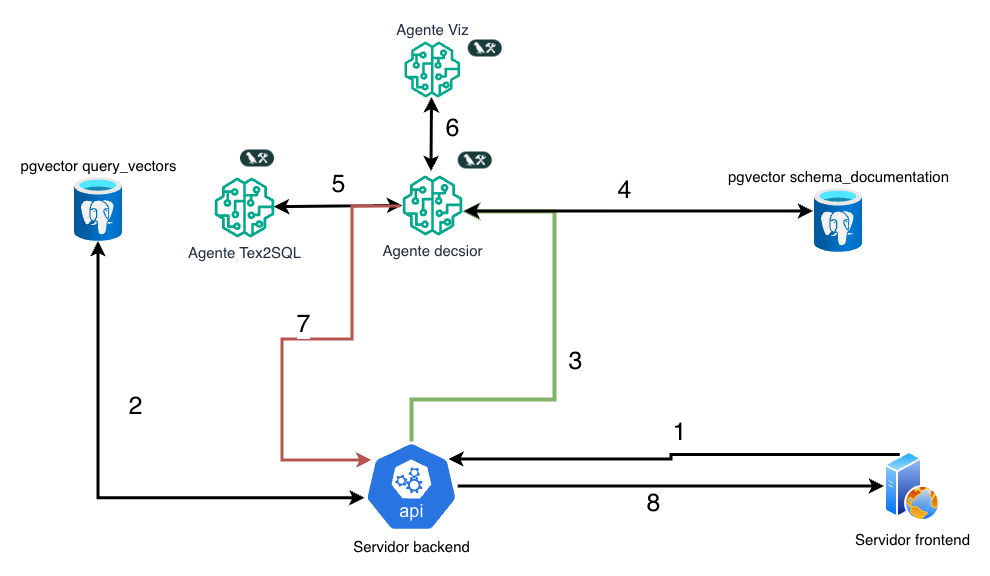
\includegraphics[width=\columnwidth]{imagenes/diagrama_arquitectura.png}
    \caption{Diagrama de arquitectura del sistema BIGENIA. Se detallan los 8 pasos de comunicación entre los agentes, el servidor y las bases de datos vectoriales.}
    \label{fig:arquitectura}
\end{figure}

El sistema BIGENIA ha sido diseñado bajo un modelo de flujo de trabajo basado en agentes (\textit{Agentic Workflow}), estructurado en diferentes componentes especializados. Como se ilustra en la Figura \ref{fig:arquitectura}, la comunicación entre las capas y los agentes sigue un proceso ordenado de 8 pasos:

\begin{enumerate}
    \item \textbf{Recepción de la consulta:} El servidor frontend (interfaz web) captura la pregunta del usuario en lenguaje natural y envía la petición HTTP al servidor backend (API REST).
    
    \item \textbf{Caché Semántico (\textit{query\_vectors}):} El servidor backend consulta la base de datos vectorial (\texttt{pgvector query\_vectors}) para comprobar si existe una pregunta semánticamente idéntica que ya haya sido procesada. Si ocurre un \textit{cache hit}, se reutiliza la consulta SQL asociada, ahorrando tiempo de procesamiento.
    
    \item \textbf{Delegación al Orquestador:} Si la consulta es nueva (\textit{cache miss}), la API transfiere la responsabilidad lógica al \textbf{Agente Decisor}, el componente central encargado de dirigir el flujo de trabajo.
    
    \item \textbf{Extracción de Contexto (\textit{schema\_documentation}):} El Agente Decisor consulta la segunda base de datos vectorial (\texttt{pgvector schema\_documentation}) para obtener los metadatos relevantes del esquema relacional (DDLs, documentación de tablas y reglas de negocio) que servirán de contexto.
    
    \item \textbf{Interacción con Text2SQL:} El Agente Decisor envía el contexto recuperado y la pregunta original al \textbf{Agente Text2SQL} (potenciado por Vanna AI) para que el Modelo de Lenguaje Grande formule la sentencia SQL correcta.
    
    \item \textbf{Decisión de Visualización (Agente Viz):} En paralelo o subsecuentemente, el Agente Decisor provee la estructura de los datos obtenidos al \textbf{Agente Viz}, quien decide la forma óptima de representarlos visualmente y genera el código JSON de configuración para Plotly.
    
    \item \textbf{Retorno de Resultados:} Una vez procesado, se transfiere la respuesta completa (incluyendo la consulta SQL, los datos y la configuración del gráfico generado) de vuelta al servidor backend, preparándola para ser enviada al cliente.
    
    \item \textbf{Respuesta Final:} El servidor backend envía este resultado consolidado al servidor frontend, donde la interfaz finalmente renderiza el gráfico interactivo y presenta la información al usuario.
\end{enumerate}

Esta arquitectura desacoplada permite que cada agente y componente de la base de datos asuma un rol altamente especializado, facilitando el mantenimiento y permitiendo futuras actualizaciones tecnológicas (como el reemplazo del modelo LLM) sin comprometer la integridad del flujo de datos completo.

Adicionalmente, se ha integrado \textbf{LangSmith} en el flujo de trabajo como plataforma de observabilidad para los modelos de lenguaje subyacentes. Esta herramienta resulta fundamental para monitorear, rastrear y depurar las ejecuciones de los agentes en tiempo real. Gracias a LangSmith, es posible analizar el rendimiento de los \textit{prompts}, medir los tiempos de latencia, auditar el consumo de tokens y detectar anomalías o alucinaciones durante la generación de sentencias SQL y gráficos, garantizando así la calidad y confiabilidad continua de las respuestas de BIGENIA.

\subsection{Agente Decisor}
Lorem ipsum dolor sit amet, consectetur adipiscing elit. Sed do eiusmod tempor incididunt ut labore et dolore magna aliqua. Ut enim ad minim veniam, quis nostrud exercitation ullamco laboris nisi ut aliquip ex ea commodo consequat. Duis aute irure dolor in reprehenderit in voluptate velit esse cillum dolore eu fugiat nulla pariatur. Excepteur sint occaecat cupidatat non proident, sunt in culpa qui officia deserunt mollit anim id est laborum.


\subsection{Agente visualizador}
Lorem ipsum dolor sit amet, consectetur adipiscing elit. Curabitur pretium tincidunt lacus. Nulla gravida orci a odio. Nullam varius, turpis et commodo pharetra, est eros bibendum elit, nec luctus magna felis sollicitudin mauris. Integer in mauris eu nibh euismod gravida. Duis ac tellus et risus vulputate vehicula. Donec lobortis risus a elit. Etiam aliquet massa et lorem. Mauris dapibus lacus auctor risus.


\subsection{Agente de base de datos}
Lorem ipsum dolor sit amet, consectetur adipiscing elit. Phasellus imperdiet, nulla et dictum interdum, nisi lorem egestas vitae scelerisque enim ligula venenatis dolor. Maecenas nisl est, ultrices nec congue eget, auctor vitae massa. Fusce luctus vestibulum augue ut aliquet. Nunc sagittis dictum nisi, sed ullamcorper ipsum dignissim ac. In at libero sed nunc venenatis imperdiet sed ornare turpis. Donec vitae dui eget tellus gravida venenatis.


\subsection{Interfaz de usuario}

La interfaz de usuario fue diseñada priorizando la simplicidad y la capacidad de respuesta inmediata. Se utilizó \textbf{React} como biblioteca principal de frontend, complementada con \textbf{Tailwind CSS} para el estilizado y \textbf{Zustand} para la gestión de estado global.

\begin{figure}[h]
    \centering
    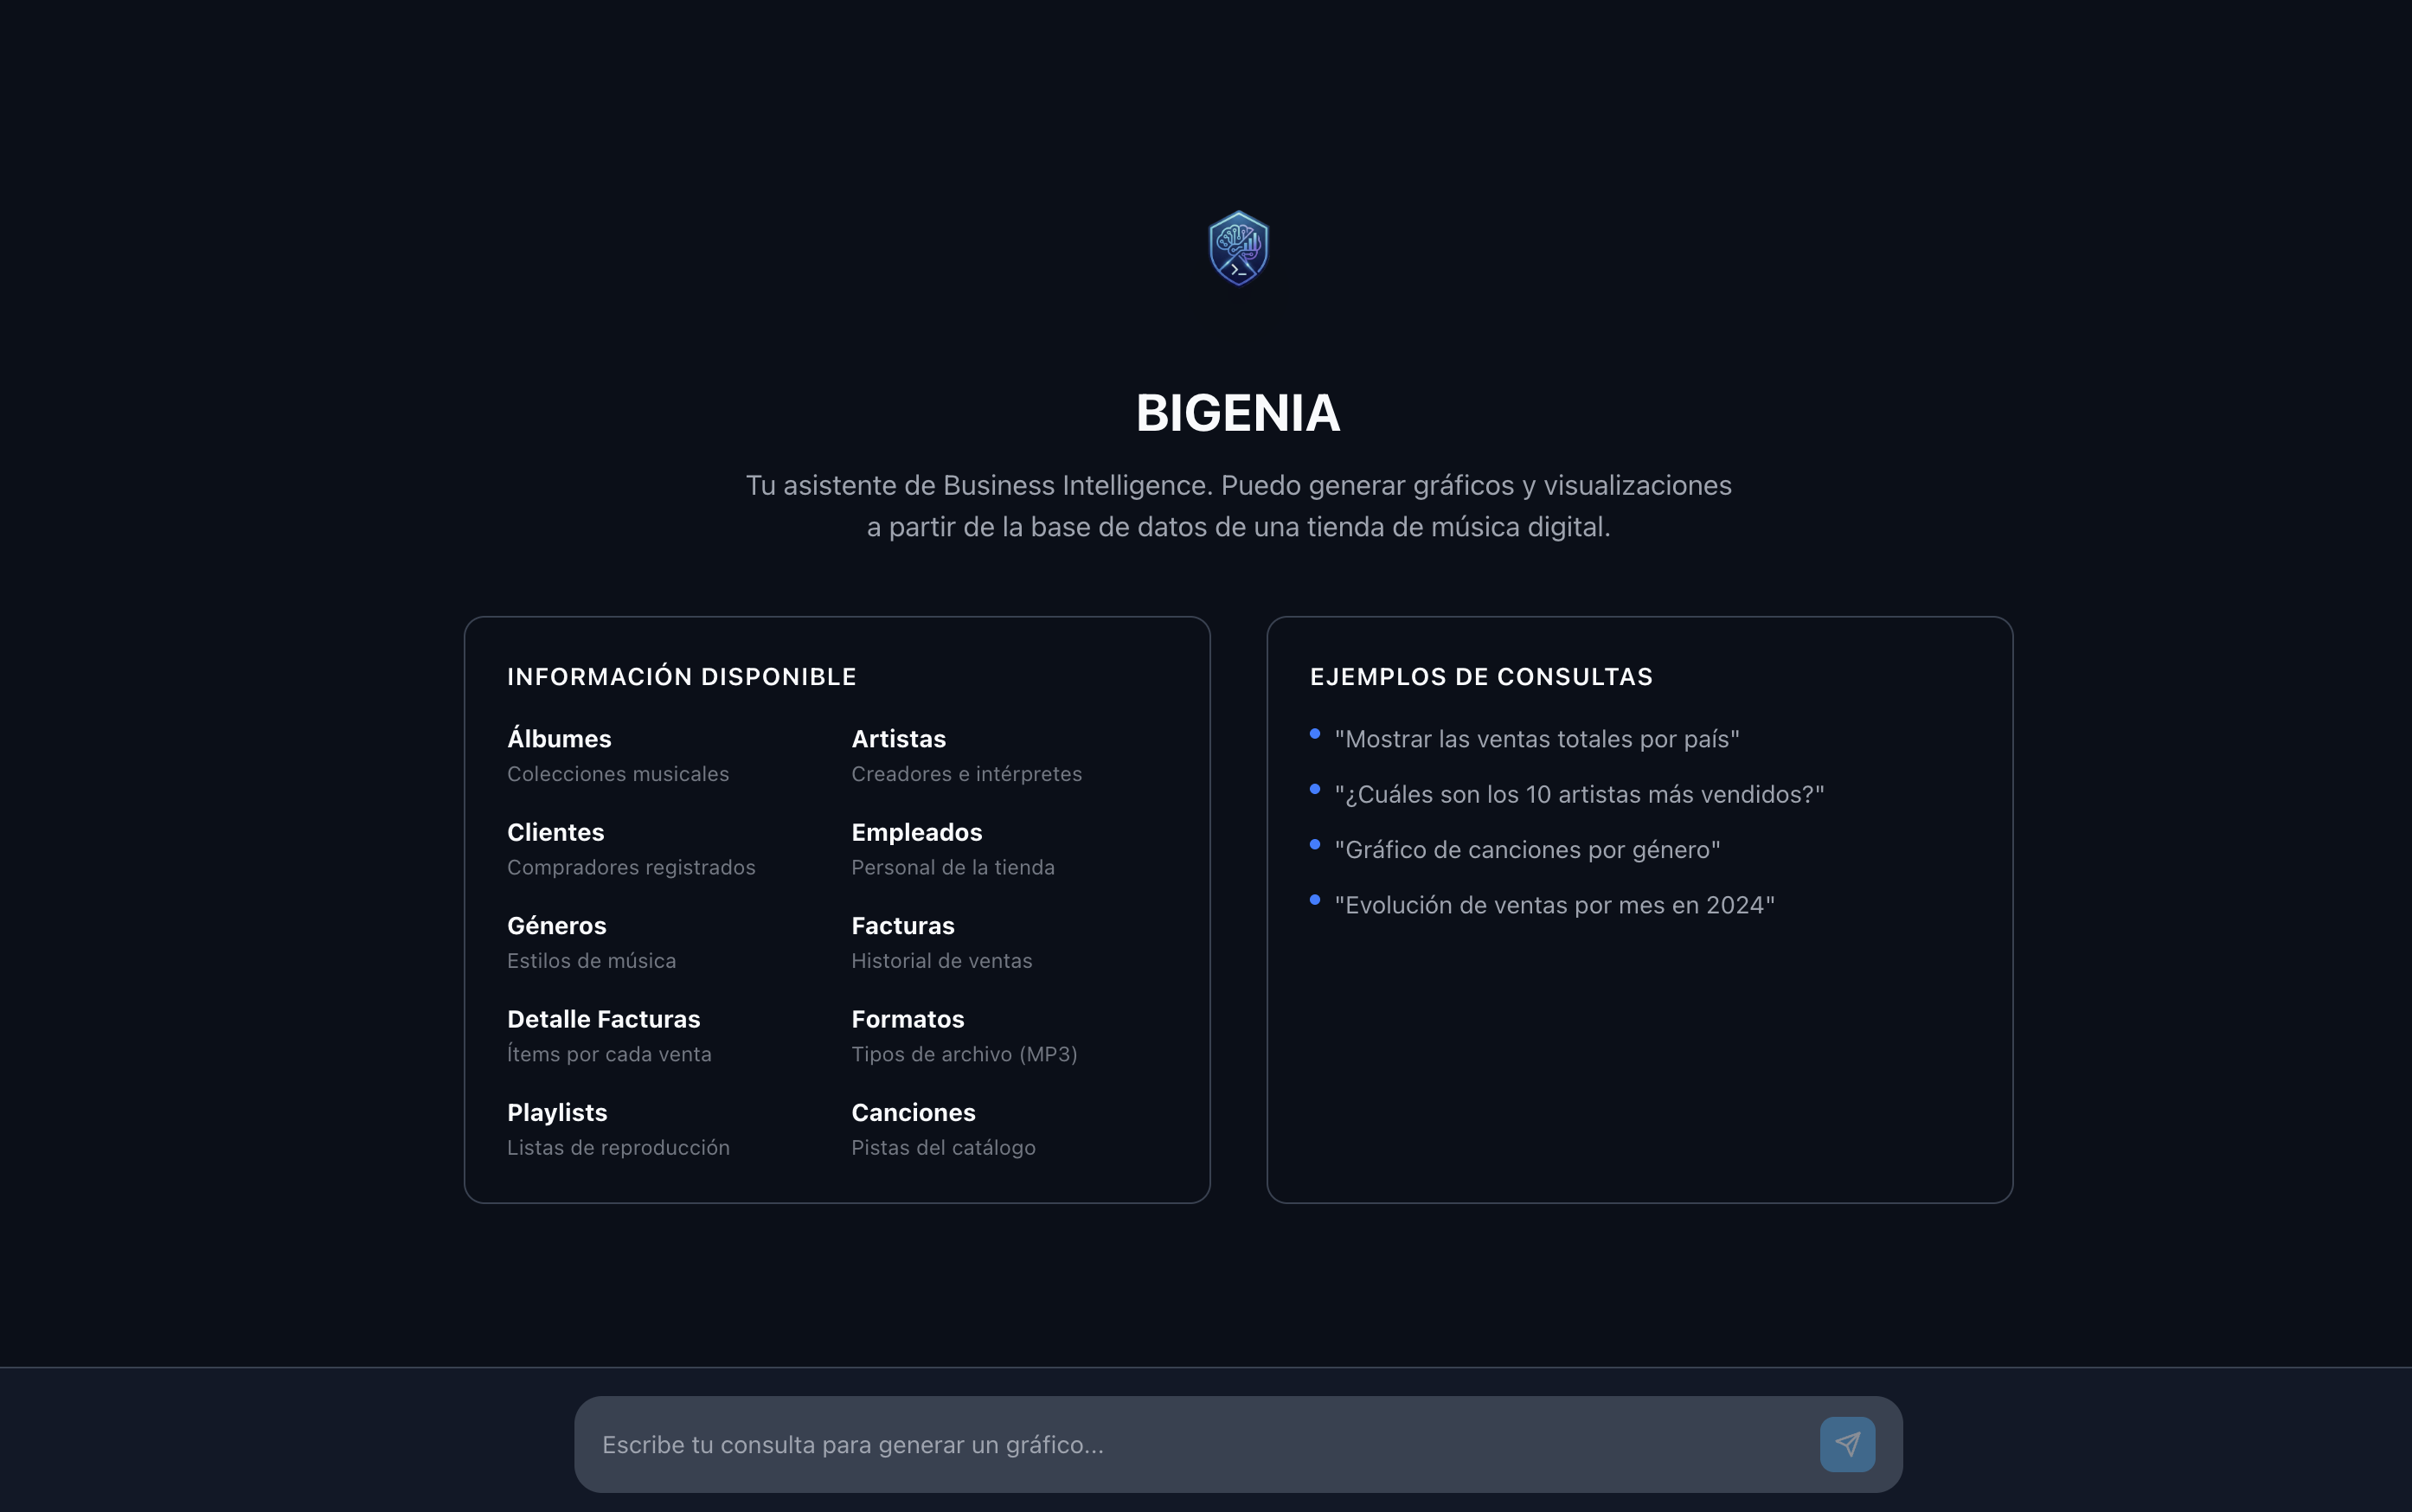
\includegraphics[width=\columnwidth]{imagenes/inicio.png}
    \caption{Pantalla de inicio de la aplicación con guía de uso.}
    \label{fig:inicio}
\end{figure}

\subsubsection{Decisiones de Diseño y UX/UI}

\begin{itemize}
    \item \textbf{Estética Moderna y Minimalista}: Se implementó un diseño con bordes redondeados, utilizando una paleta de colores coherente que soporta tanto el modo claro como el modo oscuro (ver Figura \ref{fig:grafico_claro}). Esta dualidad no es solo estética, sino que mejora la accesibilidad y reduce la fatiga visual según la preferencia del usuario.
    \item \textbf{Retroalimentación Inmediata}: Dado que la generación de gráficos mediante LLMs puede tomar varios segundos, se integraron indicadores de carga (\textit{spinners} y \textit{skeleton screens}) para mantener al usuario informado sobre el proceso en curso.
    \item \textbf{Interactividad de los Datos}: En lugar de imágenes estáticas, los gráficos se renderizan utilizando \textbf{Plotly.js}. Esto permite que el usuario pueda hacer zoom, filtrar series de datos y ver detalles exactos al pasar el cursor sobre los elementos.
\end{itemize}

\begin{figure}[h]
    \centering
    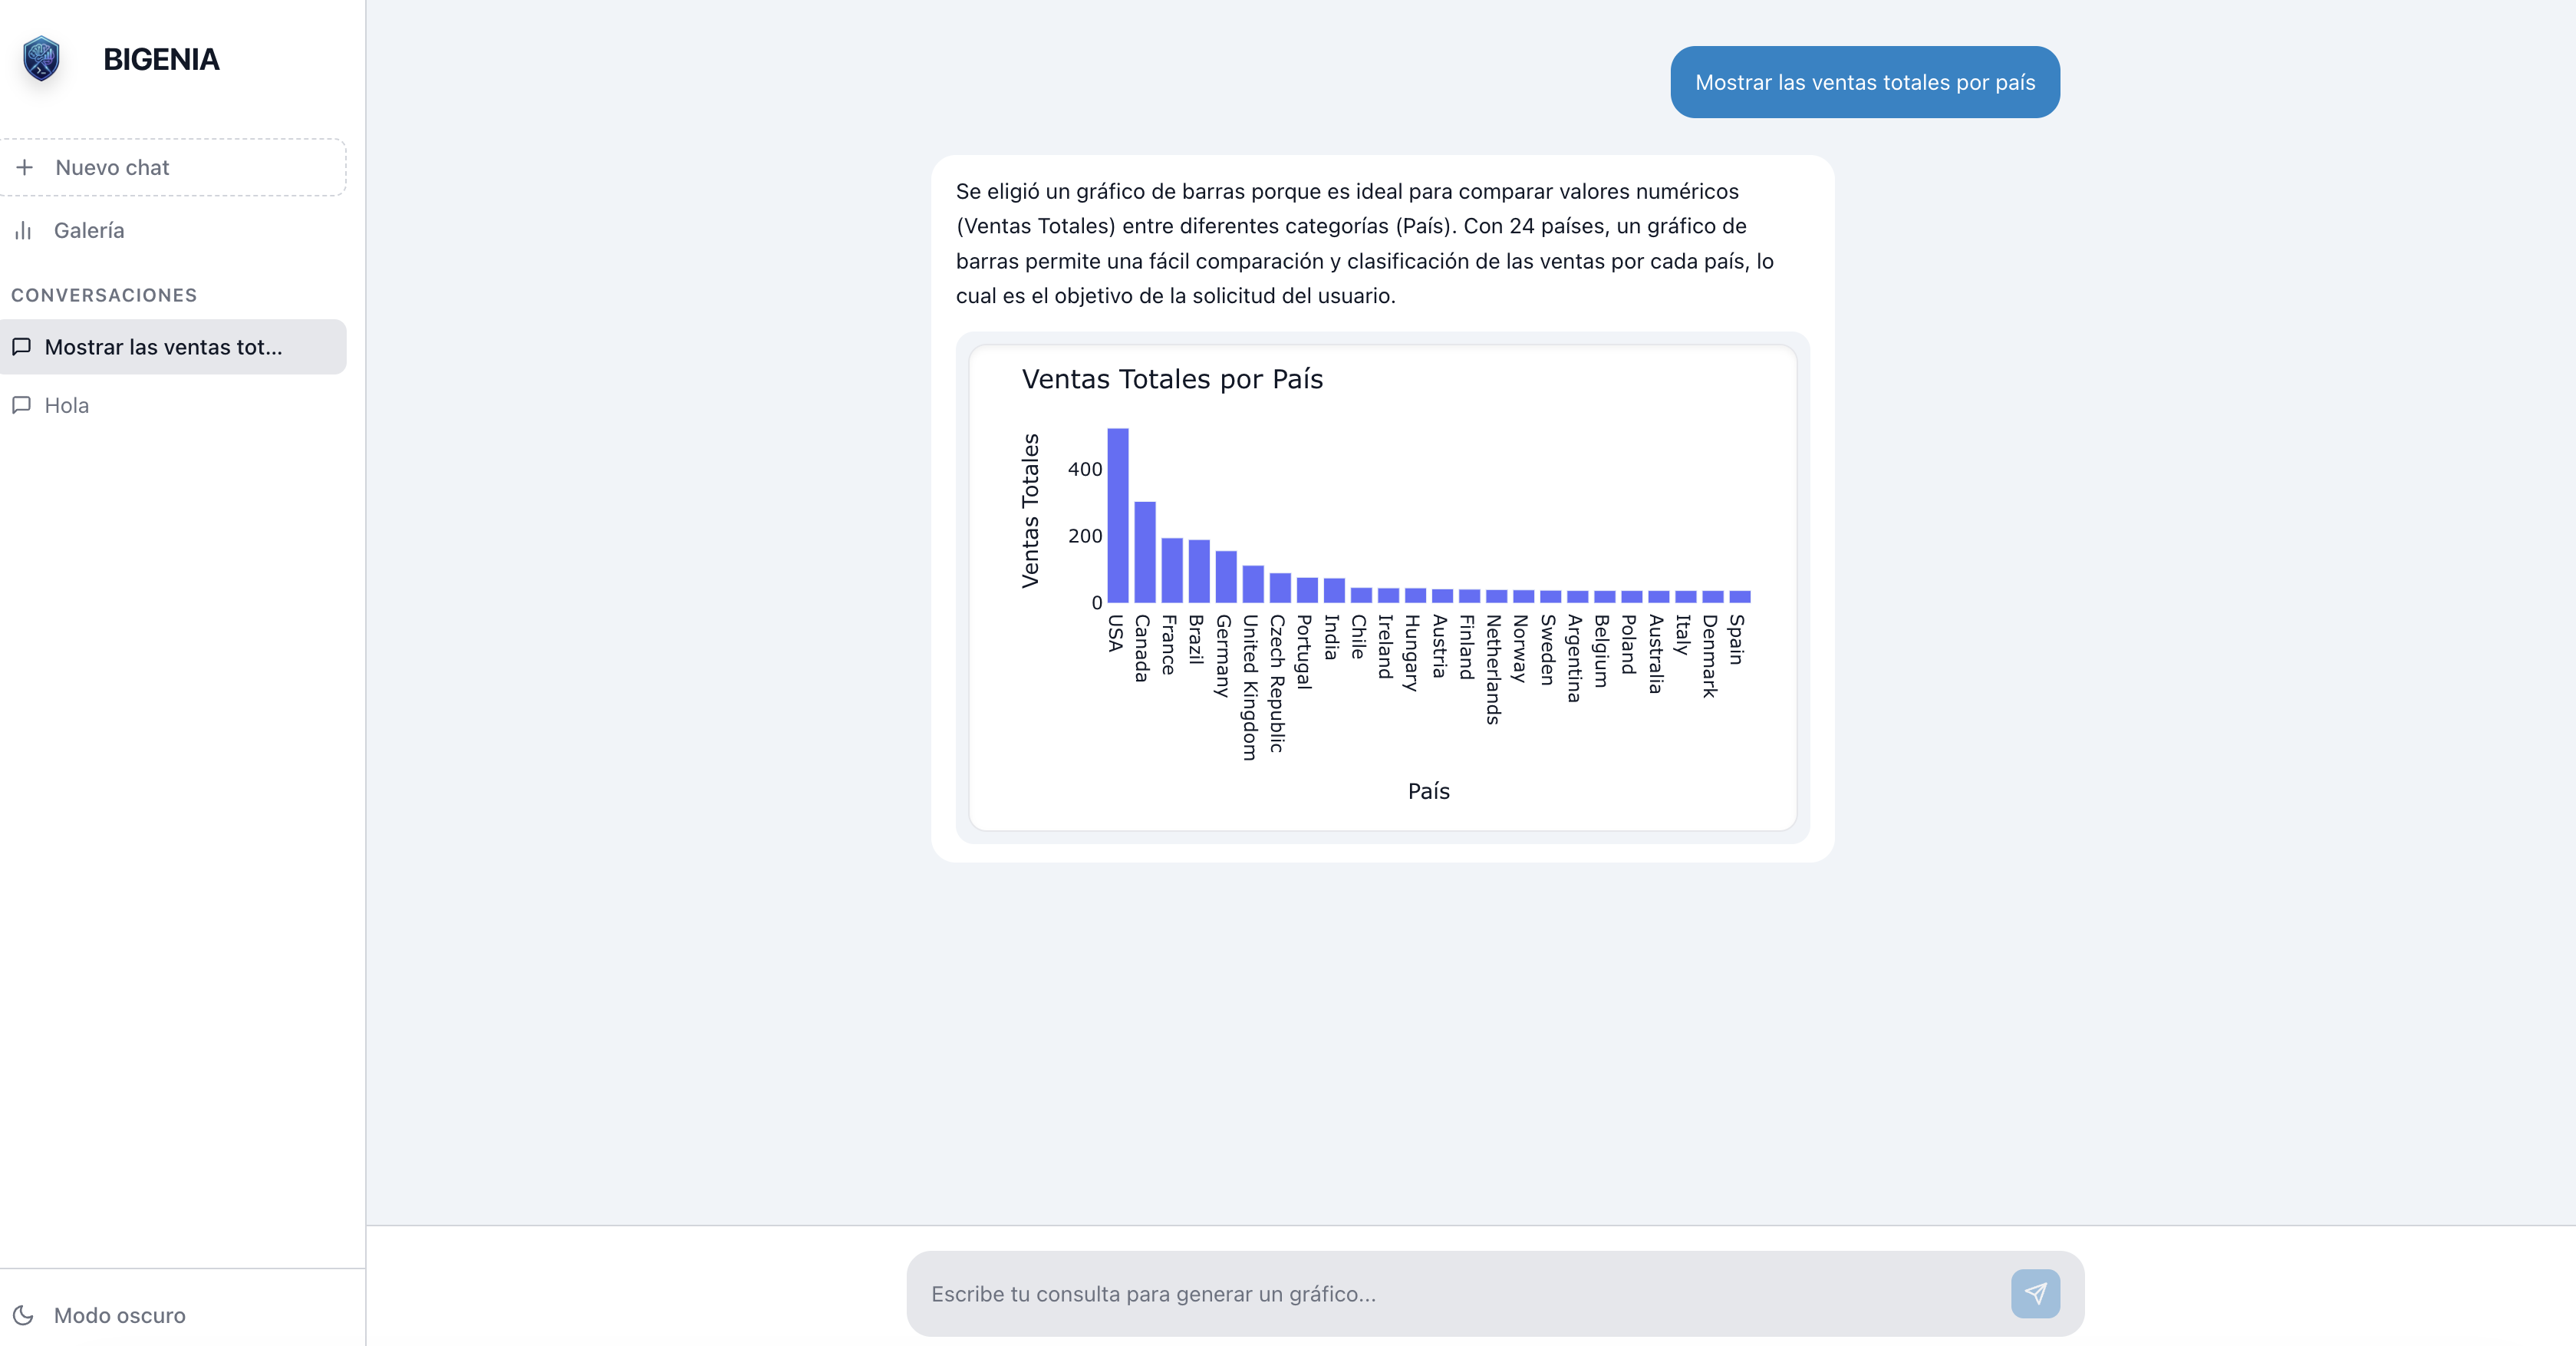
\includegraphics[width=\columnwidth]{imagenes/grafico_claro.png}
    \caption{Visualización interactiva generada en modo claro.}
    \label{fig:grafico_claro}
\end{figure}

\subsubsection{Persistencia y Organización}

Para facilitar el flujo de trabajo del analista, la aplicación cuenta con un historial de conversaciones y una \textbf{Galería de Gráficos} (Figura \ref{fig:galeria}). Esta galería permite acceder rápidamente a las visualizaciones más importantes sin tener que buscar en el historial del chat, separando la lógica de conversación de los activos visuales generados.

\begin{figure}[h]
    \centering
    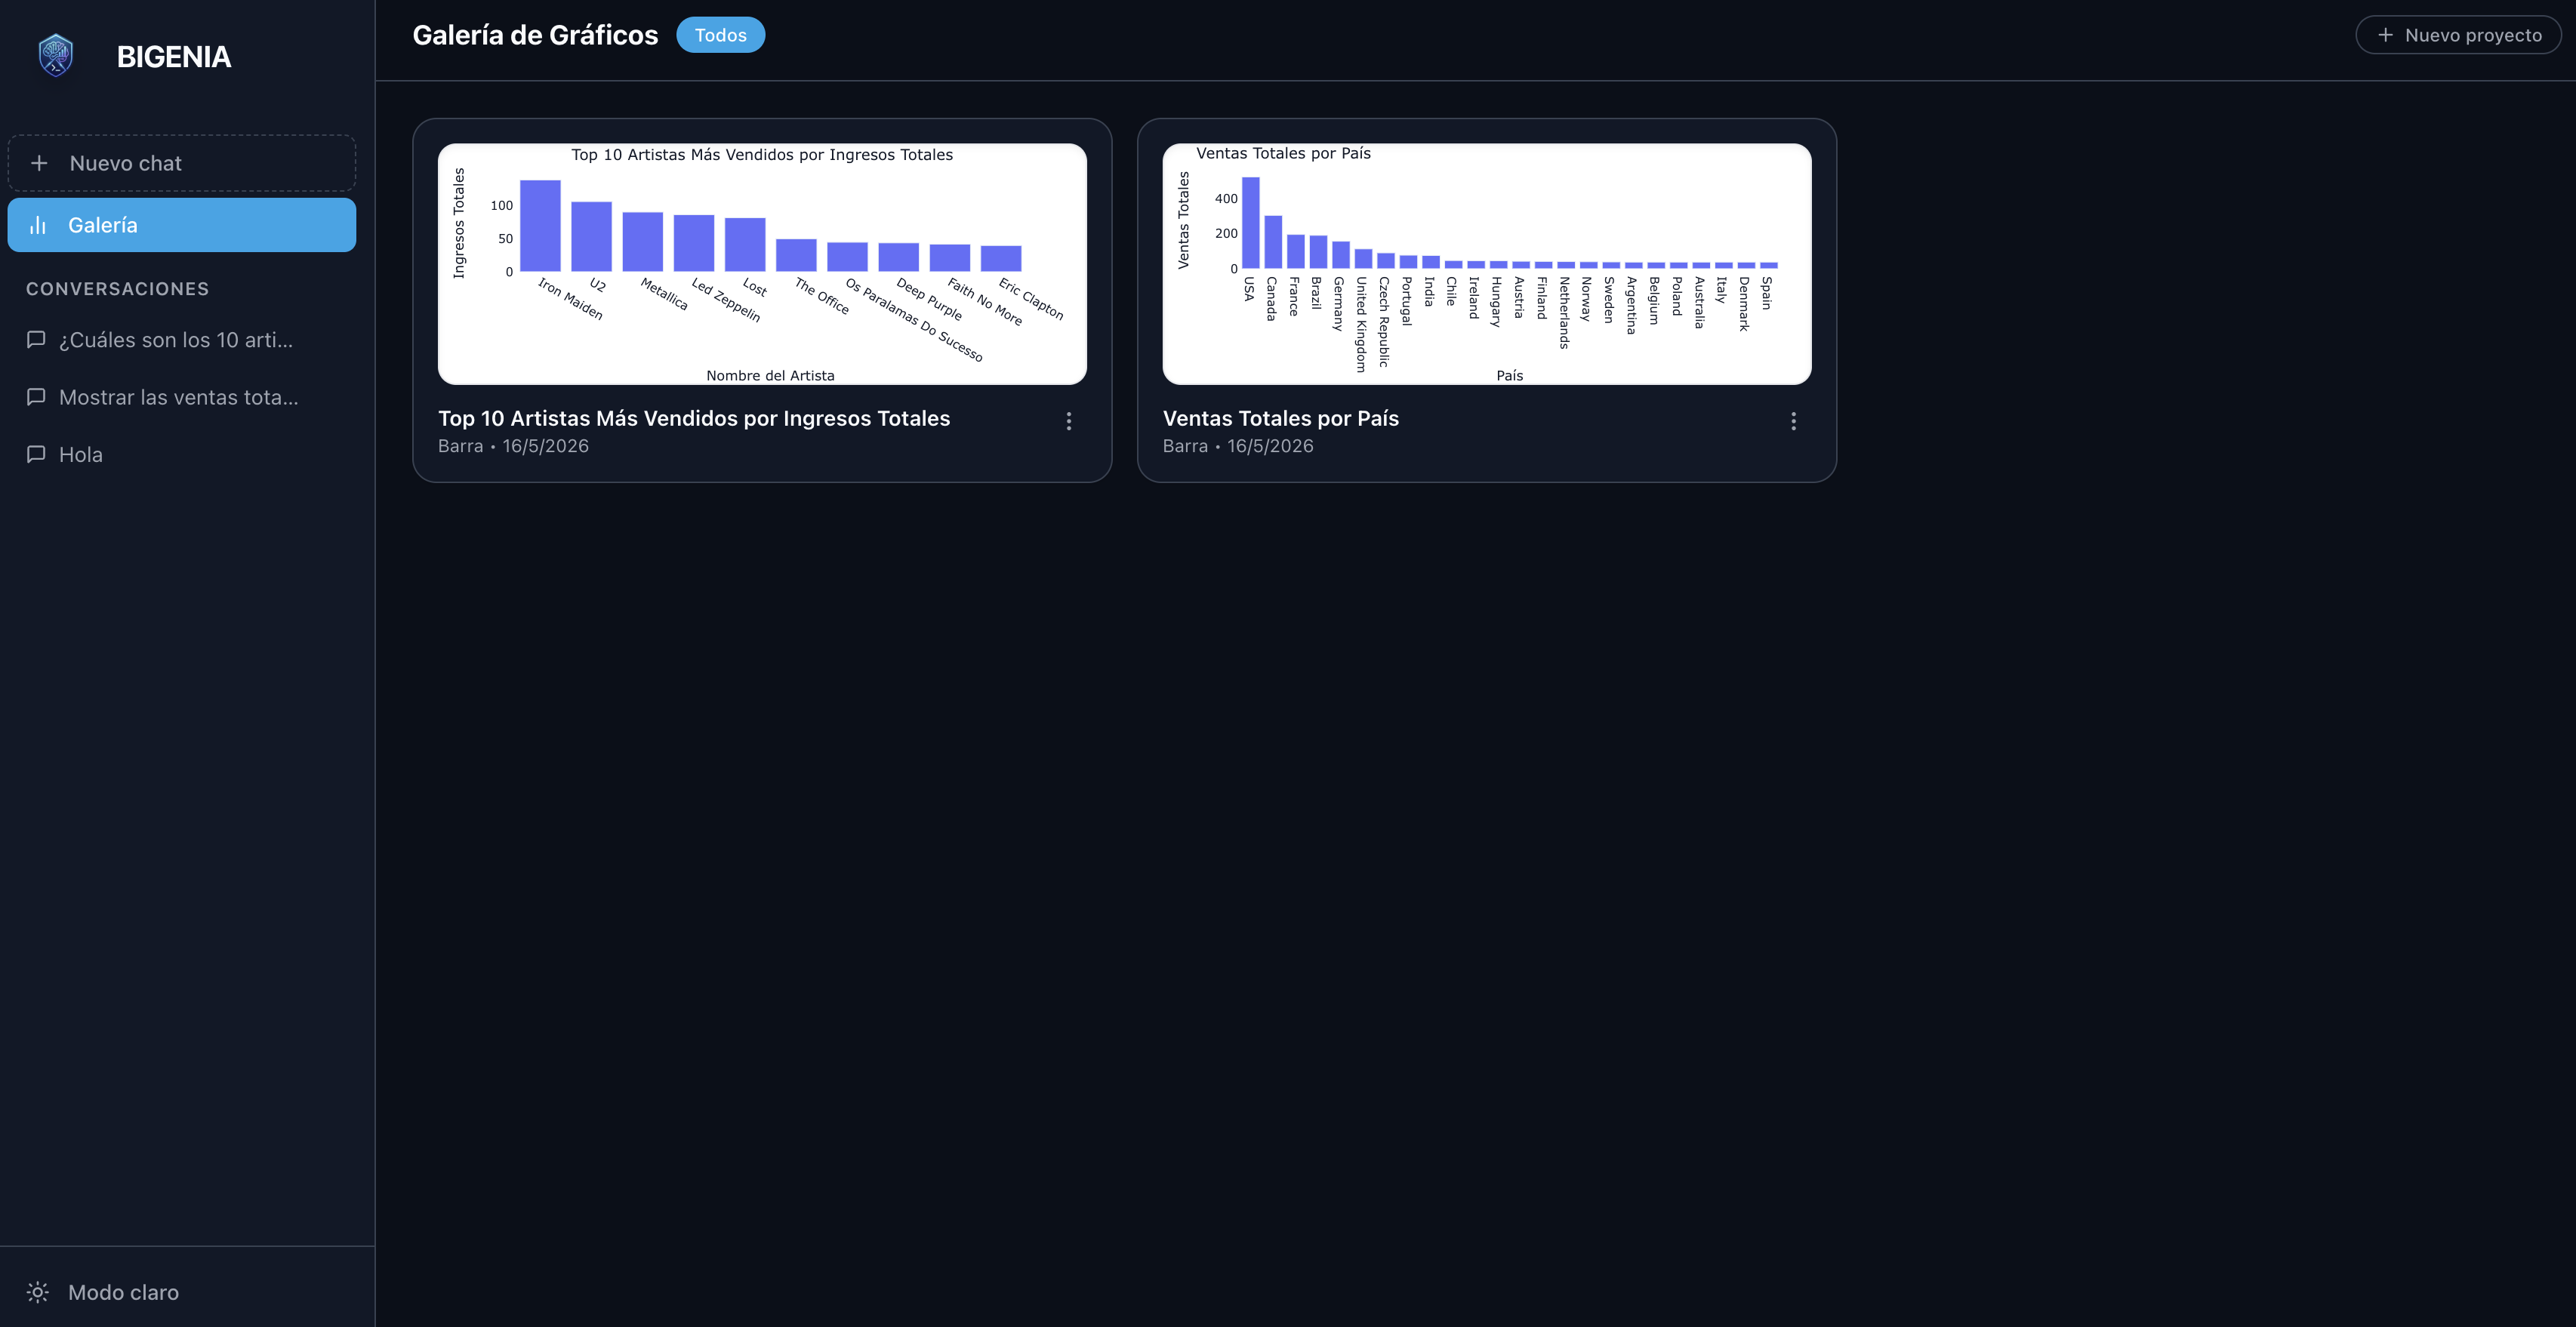
\includegraphics[width=\columnwidth]{imagenes/galeria.png}
    \caption{Galería centralizada para la gestión de activos visuales.}
    \label{fig:galeria}
\end{figure}

\subsubsection{Edición Generativa}

Una característica distintiva de la interfaz es la capacidad de modificar gráficos existentes mediante lenguaje natural. El usuario puede citar un gráfico previo y solicitar cambios específicos (ej. colores, filtros o tipos de gráfico), lo que se traduce en una experiencia de edición fluida e intuitiva (Figura \ref{fig:cambio}).

\begin{figure}[h]
    \centering
    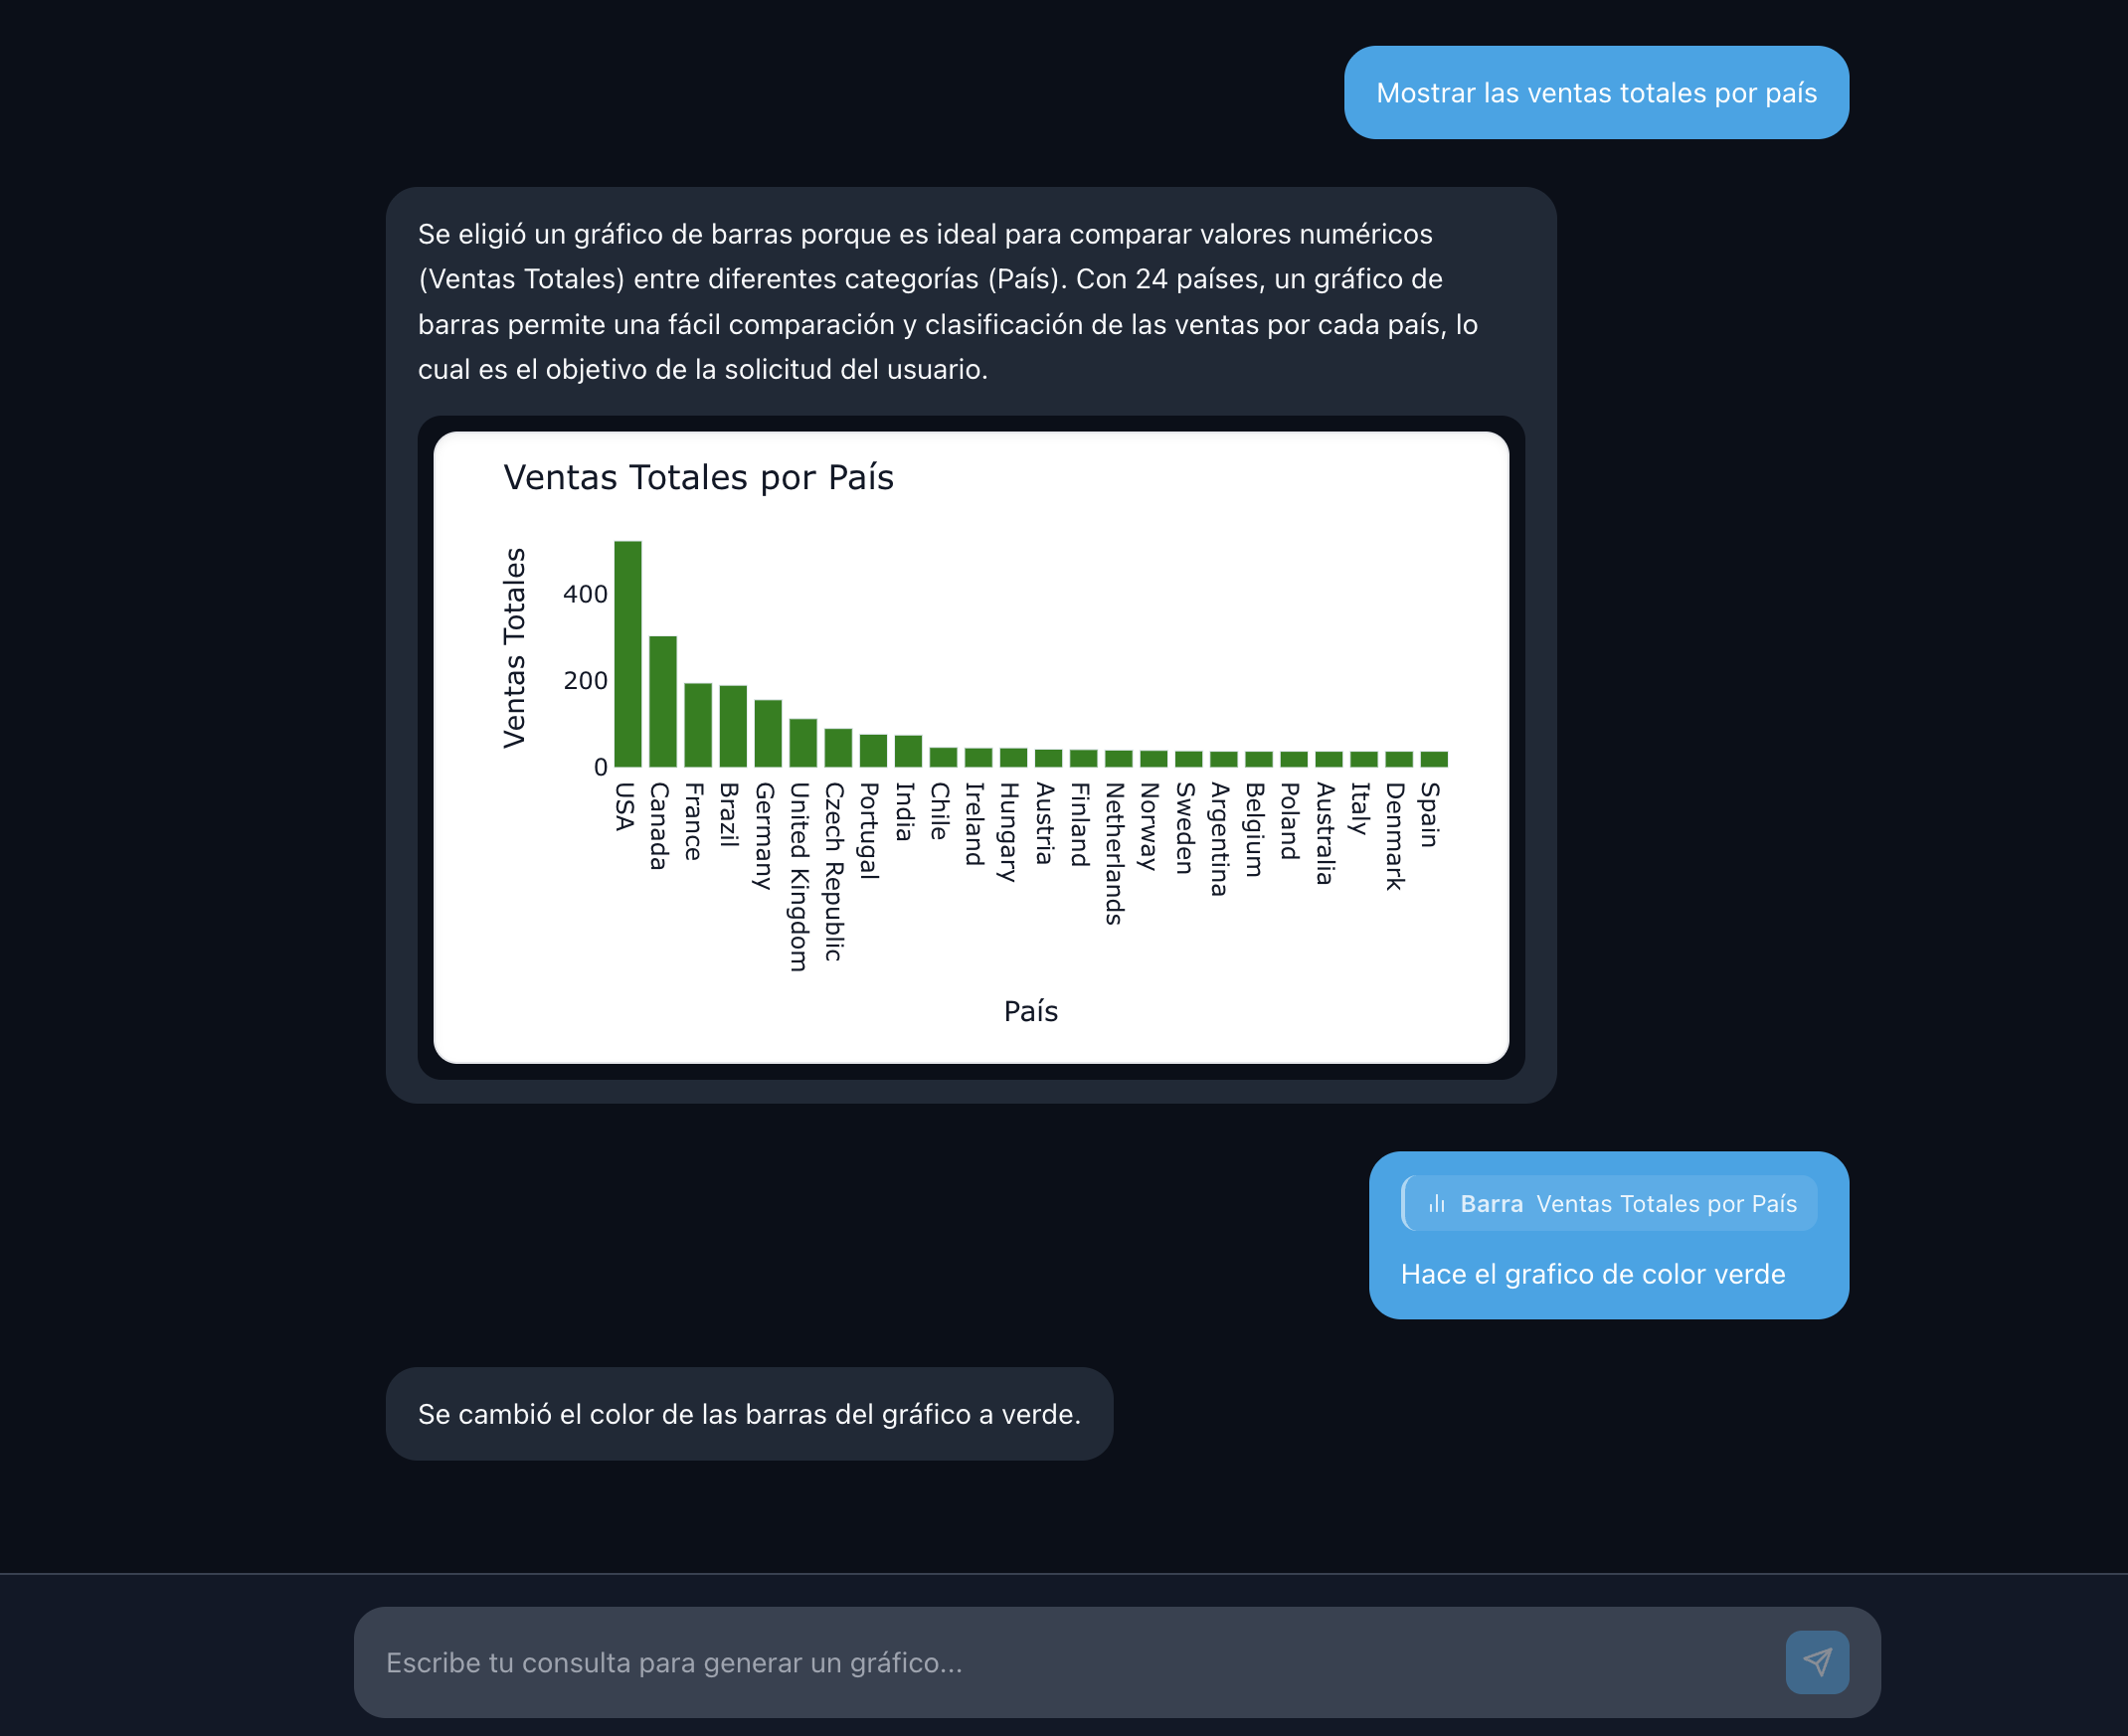
\includegraphics[width=\columnwidth]{imagenes/cambio.png}
    \caption{Flujo de edición generativa sobre un gráfico previo.}
    \label{fig:cambio}
\end{figure}
